\section{Exercises}

\begin{exercise}
\label{ex:02-circumbilliard} 
Referring to \cref{fig:02-circumbilliard}, show that every triangle has a circumbilliard, i.e., an ellipse to which it is inscribed and to which it is a billiard 3-periodic. Compute the axes of said circumbilliard with respect to triangle vertices. 
\end{exercise}

\begin{figure}
    \centering
    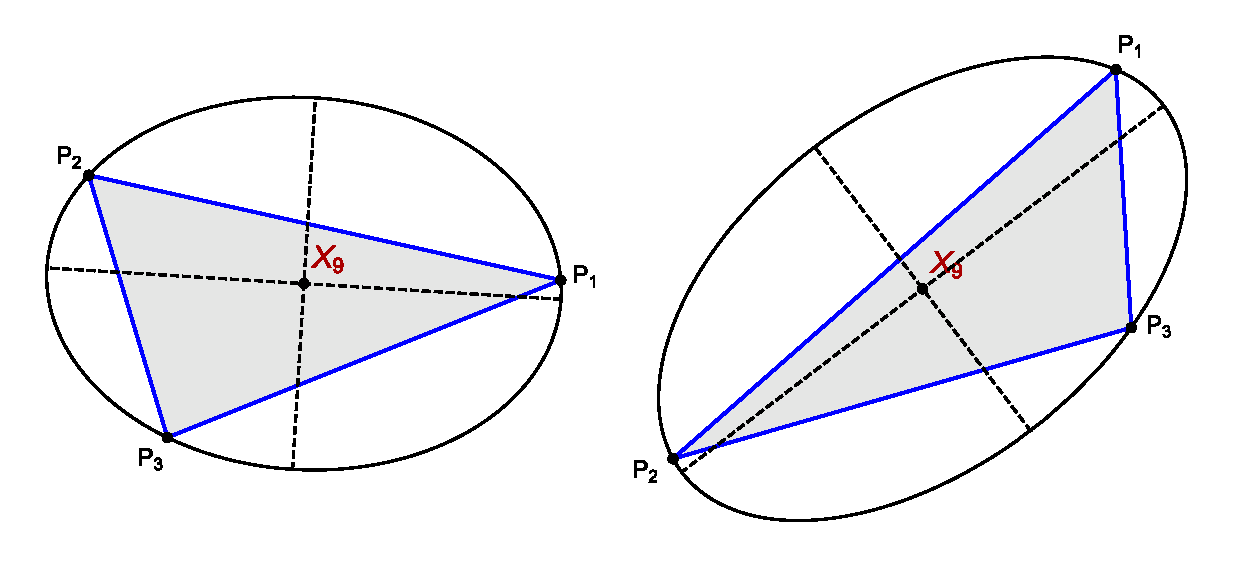
\includegraphics[width=.8\textwidth]{pics_02_910_circumplot.eps}
    \caption{Two random triangles shown with their circumbilliards. \href{https://youtu.be/vSCnorIJ2X8}{Video}}
    \label{fig:02-circumbilliard}
\end{figure}

\begin{exercise}
A pair of circles uniquely defines a {\em pencil} of coaxial circles; see \cite[Limiting Points]{mw}. The pencil contains exactly two circles which degenerate to a point, known as {\em limiting points}. Derive the location of such points for the poristic pair obtained from the image of two confocal ellipses centered at $[0,0]$ and with axes $a,b$ and $a',b'$.
\end{exercise}

\begin{exercise}
Let $\ell_1,\ell_2$ be the limiting points of the two circles which are polar images of a confocal pair $\E,\E'$ with respect to a circle centered on $f_1$. At what aspect ratio $a/b$ of $\E$ will $\ell_2$ coincide with $f_2$?
\end{exercise}

\begin{exercise}
A well-known result is that the inversion of a circle pair $\Cm,\Cm'$ with respect to a circle $\Cm_1$ centered on $\ell_1$ (resp. $\Cm_2$ centered on $\ell_2$) is a pair of concentric circles $\Cm_1'$ and $\Cm_1''$ (resp. $\Cm_1'$ and $\Cm_1''$). Prove the following lesser known result: the ratio of radii between $\Cm_1'$ and $\Cm_1''$ is the same as the ratio between $\Cm_2'$ and $\Cm_2''$. 
\end{exercise}

\begin{exercise}
Referring to \cref{fig:08-concentric-inverted}, let $\Cm,\Cm'$ be the pair of circles which are the polar image of a confocal pair of ellipses $\E,\E'$. Let $\Cm_1', \Cm_1''$ be the inversive images of $\Cm,\Cm'$ wrt to a circle centered on a focus of the ellipse pair. Prove that: (i) $\Cm_1'$ and $\Cm_1''$ are concentric with the ellipse pair and (ii) $\Cm_1'$ (resp. $\Cm_1''$) is externally tangent to $\E$ (resp. $\E'$) at its left and right major vertices.
\end{exercise}


\begin{exercise}
Prove the inversive image of billiard 3-periodics with respect to a focus-centered circle is a non-Ponceletian family inscribed in Pascal's Limaçon whose Gergonne point $X_7$ is stationary; see it \href{https://bit.ly/3edwKD7}{Live}. Indeed, this family has constant perimeter (to be shown later).
\end{exercise}

\begin{exercise}
 Consider the ellipse $x^2/a^2+y^2/b^2=1$. For a  3-periodic  billiard orbit with vertices $P_i=[x_i,y_i]$ (i=1,2,3)  show that:  

\[ 
 \left( x_2\,y_3-x_3\,y_2 \right) x_1\,
y_1+ \left(x_3\,y_1  - x_1\,y_3\right) x_2\, y_2+ \left( x_1\,y_2-x_2\,y_1 \right) x_3
\,y_3=0
\]

\end{exercise}

\begin{exercise} For a  3-periodic  billiard orbit with vertices $P_i=[x_i(t),y_i(t)]$ (i=1,2,3)
Let $C_i(t)=[1/x_i(t),1/y_i(t)]$. 
%Here $P_i(t)=[x_i(t),y_i(t)]$.

Show that the polygon $\{C_1(t),C_2(t),C_3(t)\}$ is a segment that can be bounded or unbounded.
 \label{exe:chap02-inverse-envelope}
\end{exercise}

\begin{exercise} Which simple or self-intersected $N$- gon (closed polygon with $N$ vertices and $N$ sides) can be an orbit on an elliptic billiard? 

 For $N=4$ only the parallelogram can be a non self-intersected orbit on an elliptic billiard, see \cite{connes07}. For the analysis of self-intersected $4-gons$ see \cite{garcia2020-self-intersected}.
\end{exercise}

\begin{exercise}
 Consider a 3-periodic billiard orbit and its antipodal orbit. Show that the six points of intersections of the two triangles are contained in a stationary confocal ellipse $\mathcal{E}_h$: $x^2/a_h^2+y^2/b_h^2=1$ where:


\begin{align*}
	a_h=& {\frac { \left(  \delta -b^2\right) \left( {a}^{2}+{b}^{2}+2\,\delta \right)\sqrt {2\delta-{a}^{2}-{b}^{2} 
			 }  }{3 \left( {a}^{2}-{
				b}^{2} \right) ^{2}}}\\
	%
b_h=&  \,{\frac {\left( {a}^{2}-\delta \right)  \left( {a}^{2}+{b}^{2}+2\,\delta \right) \sqrt {2\delta -{a}^{2
			}-{b}^{2} } }{3 \left( {a}^{2}-
		{b}^{2} \right) ^{2}}}
%
\end{align*}
Conclude that the pair of ellipses $\{\mathcal{E}_h, \mathcal{E}_1\}$ is a billiard pair having all orbits of period 6.
Also show that the pair $\{\mathcal{E} , \mathcal{E}_h \}$ defines a zig-zag billiard and that the orbits have period 12 and  that the perimeter is  constant. %See Fig. \ref{fig:6zigzag}.
\end{exercise}




